\documentclass[a4paper,11pt]{article}

\usepackage[frenchb]{babel}
\usepackage[utf8]{inputenc}
%\usepackage{verbatim}
\usepackage{graphicx}

\begin{document}
\title{Compte Rendu du TD numéro 3 (Suite et Fin) puis Compte Rendu du TD numéro 4 de l'équipe Eirb'reteau}
\date{Pour le 13 octobre}
\maketitle

\begin{center}
  Coordinateur :  Lionel Adotevi \\
  Tandem 1 : Pierre Gaulon, Reda Boudjeltia \\
  Tandem 2 : Victor Dury,  Aurélien Nizet \\
\end{center}
\maketitle

\section*{Boutez vos neurones (partie 4 du TD3)}
Tout d'abord, nous avons commencé par modifier les trois états DEHORS, ASSIS et DEBOUT. Pour les partager, nous en avons fait des variables d'instance (static), et constantes (final), pour qu'elles ne soient plus modifiées. Ces trois variables de la classe EtatPassager sont des instances de la classe EtatPassager elle-même, instanciées par le constructeur par défaut, lors de la compilation de cette classe. En réalité, ce qui différencie ces trois états, c'est simplement leur référence, leur adresse mémoire qui est différente. Il n'y a plus d'état courant. On a donc supprimé les anciens constructeurs, et toutes les références à l'état courant. Pour toutes les méthodes d'accès de cette classe, on compare la référence de la classe utilisée (this), avec les références DEBOUT, ASSIS, DEHORS. Par exemple this==DEHORS va caractériser l'état estExterieur() d'un PassagerStandard. De même pour les autres méthodes d'accès d'état. Pour changer d'état, il suffit simplement de renvoyer l'adresse de l'état ciblé. Par exemple pour faire assoir un PassagerStandard, il suffit de faire return ASSIS;. La méthode toString() a aussi dû être changée. En effet, le switch case n'était pas compatible avec des comparaisons de références, on l'a alors changé en succession de if. Enfin, comme nous n'avions plus de constructeur de EtatPassager, mais qu'il faut bien initialiser un état par défaut lors de la construction d'un PassagerStandard, nous avons créé une nouvelle méthode de classe static public EtatPassager construct(), qui renvoie la référence de DEHORS. Ainsi, il est possible d'initialiser un EtatPAssager.

\section*{Recette}
Commande pour lancer les tests unitaires dans le répertoire tstPassager : \\
\$ java -ea -cp build-tstPassager/:build/ tec.LancerTests
Commande pour lancer les tests unitaires dans le répertoire tstAutobus : \\
\$ java -ea -cp build-tstAutobus/:build/ tec.LancerTests

Il faut les exécuter séparément, car les tests d'Autobus dépendant du faussaire de PassagerStandard, et de la classe Autobus, et les tests de PassagerStandard dépendent du faussaire de Autobus, et de la classe PassagerStandard. Pour exécuter correctement les tests, il est donc nécessaire de ne pas mélanger les faussaires (notamment lors des tests de messages envoyés). Ces faussaires sont dans deux répertoires différents, et donc il faut séparer ces répertoires dans l'option -classpath, ce qui n'aurait pas été possible en une seule exécution.

Commande de compilation de la classe Simple :\\
\$ javac -d build/ src/* \&\& javac -d build/ -cp build/ recette/Simple.java

Commande d'exécution de la classe Simple : \\
\$ java -cp build/ Simple

\newpage
\begin{centering}
{\textbf{TD4}}


Dans ce TD nous allons user d'abstractions pour \og améliorer \fg le code, changer les fonctionnalités, ceci par l'introduction
de nouvelles classes (interfaces) et autres manipulations.

\end{centering}

\section{Programmer avec des abstractions}

Dans cette partie, nous allons introduire deux abstractions, \textbf{Bus} et \textbf{Passager} qui sont des interfaces java. Cela implique donc des
modifications dans les classes \textbf{Autobus} et \textbf{PassagerStandard} et leur faussaires: Il faut lier ces classes aux interfaces avec une relation
de type/sous-type qui est exprimée dans le code par une \textbf{implements}.

L'importance de cette relation de type/sous-type à savoir \textbf{implements} ici, est la réutilisabilité du code. En effet, les interfaces sont réutilisables.

\subsection{Les interfaces Passager et Bus}

La méthode \textbf{toString()} n'a pas besoin d'être déclarée dans ces interfaces car elle est déjà déclarée dans la classe Object et toutes nos classes ont
un lien avec cette classe Object.

Nous n'avons eu aucune erreur lors de la compilation des interfaces.

\subsection{Remaniement des classes Autobus et PassagerStandard}

Comme mentionné plus haut, dans cette partie, nous avions à modifier le code de \textbf{Autobus} et \textbf{PassagerStandard} de sorte à utiliser nos interfaces.
La relation de type/sous-type nécessaire est bel et bien \textbf{implements} car on a une interface java. Ainsi on a une relation implements entre AutoBus et Bus
et une autre entre PassagerStandard et Passager.

Le type d'erreurs rencontré est: "in interface cannot be applied to given types: bus.demanderSortie(this); required passager" si l'implements ne concernait pas la
bonne interface.

Pour compiler et exécuter la nouvelle version de la classe \textbf{Simple} on a fait: \\
\$ javac -d build/ src/* \&\& javac -d build/ -cp build/ recette/Simple.java \\
\$ java -cp build/ Simple 

\subsection{Remaniement des tests unitaires}

Toutes les modifications de cette partie ont été faites (voir code). En effet, le classe FauxBus a une relation implements avec la classe Bus et FauxPassager avec 
Passager. Et ensuite il était important de vérifier que les constructeurs avaient le même nom que nos classes.

\subsection{Réorganisation des répertoires tests}

Les modifications ont été faites au niveau du code. De plus, nous n'avons pas eu à supprimer les répertoires inutiles car nous n'avons pas copié intégralement les 
fichiers du TD3. Nous n'avions pris que ce dont nous avions besoin.

Les 4 classes visibles sont: Autobus, PassagerStandard, Bus, Passager.

\begin{figure}[h]
   \caption{Diagramme de classe 1}
   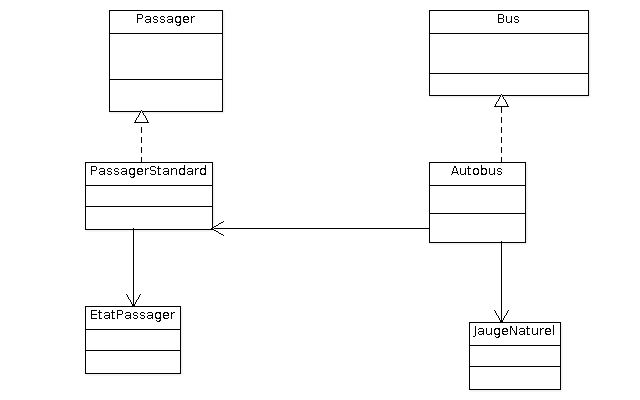
\includegraphics[scale=0.6]{figure1.png}
\end{figure}

\section{Portée et dépendances de compilation}

Pour limiter les dépendances de compilation, il nous est proposé de remplacer les interfaces par des classes abstraites et de modifier la portée des méthodes
internes au paquetage. Mais cette solution n'est pas satisfaisante en terme de dépendance. Le problème se situe au niveau de la différence entre une classe
abstraite et une interface. Le lien entre interface et abstract est étroit, car dans les deux cas, nous n'écrivons pas de code dans les fichiers. Cependant, dans 
une classe abstraite, nous écrivons les méthodes nécessaires à l'implémentation des classes filles, alors que l'interface sert de généralisation afin d'implémenter
plusieurs représentations du même type. Ainsi, utiliser des classe abstraite au lieu d'interface risquerait d'augmenter les dépendances.

Par la suite, on introduit donc deux interfaces publiques, Usager et Transport rendant ainsi Passager et Bus internes au paquetage. Cela entraîne donc des
remaniements.

Dans la méthode \textbf{monterDans(Transport t)} de PassagerStandard, on utilise les méthodes \textbf{aPlaceAssise()}, \textbf{aPlaceDebout()}, 
\textbf{demanderPlacerAssise()} et \textbf{demanderPlaceDebout()}. Or, l'interface Transport ne dispose que des méthodes \textbf{aPlaceAssise()} et 
\textbf{aPlaceDebout()}. Il est impossible de demander une place debout (et assise) à un Transport, qui ne dispose pas de cette méthode. Ainsi, pour l'utiliser on 
est alors obligé de convertir ce Transport t en Bus b, car un Bus \textbf{"est-un"} Transport, et dispose de ces deux méthodes demanderPlaceDebout() et 
demanderPlacerAssise().

Les interfaces Bus et Passager sont internes au paquetage. Mais les classes concrètes Autobus et PassagerStandard, sont quant à elles publiques, puisqu'on doit 
laisser l'accès à leurs constructeurs, utilisés par le client. Or, les méthodes définies dans Bus et Passager sont publiques, et implémentées dans les classes 
concrètes publiques PassagerStandard et Autobus. Ainsi, ces méthodes déclarées dans les interfaces internes au paquetage sont accessibles par le client au travers 
des classes concrètes publiques qui les implémentent.

\section{Les classes concrètes}

Les deux méthodes de la classe FabriqueTec sont :\\
public static PassagerStandard fairePassagerStandard(String nom, int arret)\\
public static Autobus faireAutobus(int nbPlaceAssise, int nbPlaceDebout)

La première contrainte est que cette classe ne doit pas être instanciée. Cela est réalisé, en passant les deux méthodes en static (méthodes de classe), et en 
n'important pas la classe tec.FabriqueTec dans le fichier du client, mais en utilisant directement ces deux méthodes d'instance : \\
Transport serenity = tec.FabriqueTec.faireAutobus(1,2); et \\
Usager kaylee = tec.FabriqueTec.fairePassagerStandard("Kaylee", 5); .

La deuxième contrainte est que cette classe ne doit pas servir de classe de base. Cette contrainte est réalisée simplement en ajoutant le mot-clé final devant la 
classe : aucune classe de pourra l'étendre, elle ne pourra pas être héritée.

Diagrammes de classes:
\begin{figure}[h]
   \caption{Diagramme de classe concrète non publique}
   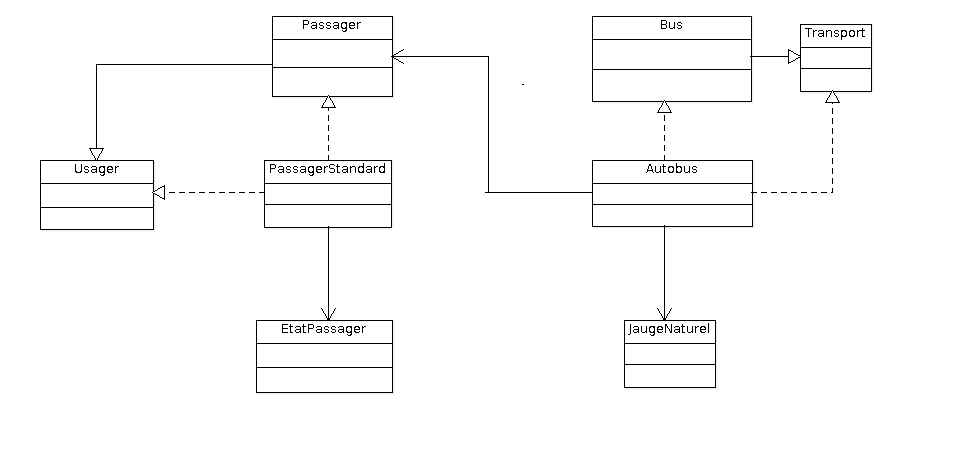
\includegraphics[scale=0.9]{nonPublique.png}
\end{figure} \\

\begin{figure}[!h]
   \caption{Diagramme de classe concrète publique}
   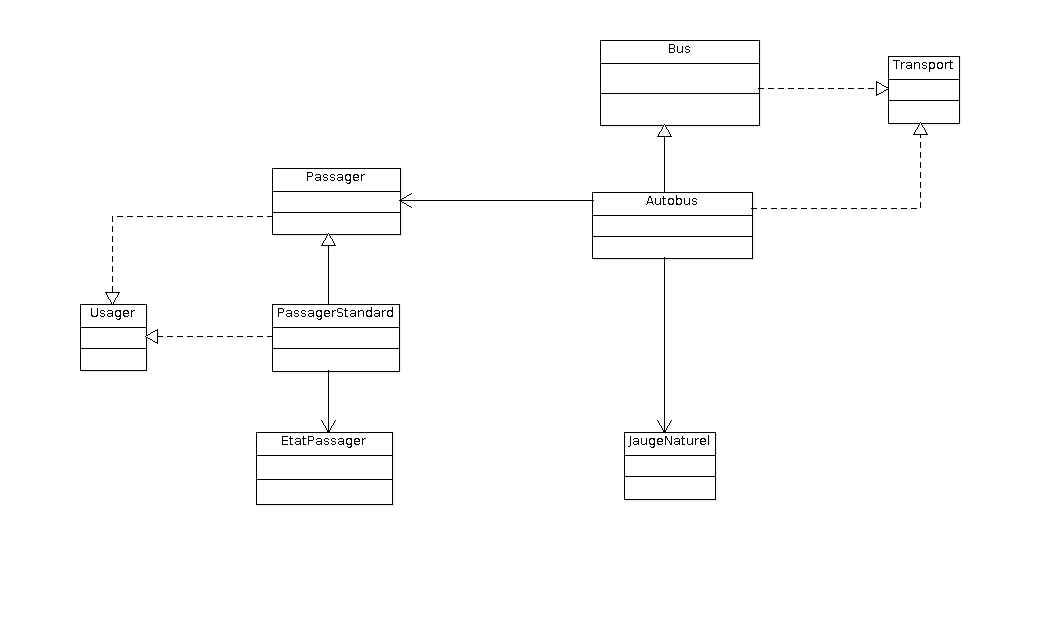
\includegraphics[scale=0.9]{Publique.png}
\end{figure}

\newpage
\section{Boutez vos neuronnes}

Utilisation de l'introspection:

\noindent try\{ \\
  \indent lancer(TestJaugeNaturel.class); \\
\} catch (Exception e)\{ \\
  \indent System.out.println("Erreur lors des tests : "); \\
  \indent e.printStackTrace(); \\
\}

\section{Commentaires}
\subsection{Commentaire de Pierre}
La chose que je retiendrai de ce TD est le soin qu'il faut porter à l'étude de la portée des différentes méthodes de nos classes. Il faut qu'elles soient suffisamment minimales pour respecter l'abstraction, mais qu'elles permettent tout de même le bon fonctionnement du logiciel. Ici cela a entraîné de nombreux remaniements et modifications, pour arriver à des portées convenablement posées. Et ça n'a pas été évident pour nous d'arriver à un programme qui compilait sans erreurs de portée, puisqu'on on a passé pas mal de temps à y arriver.

\subsection{Commentaire de Reda}
Grâce à ce TD, j'ai appris à manipuler les interfaces et les classes abstraites. Cela, m'a permis de faire la différence entre l'utilité d'une interface qui pour moi n'était qu'une simple classe 100\% abstraite et une classe abstraite. J'ai pu aussi me rendre compte des limites de java et comment il est possible de les contourner sur les questions d'héritage.

\subsection{Commentaire d'Aurélien}
J'ai trouvé ce TD assez particulier puisque nous n'avons pas eu à écrire énormément de code, c'était notamment de la réorganisation et du remaniement de code. 
Il m'a fait comprendre que derrière le langage java il y avait une part importante de théorie pour la gestion des classes et méthodes publique ou privé ainsi que 
pour tout ce qui est de la gestion du code, dans le but de créer un logiciel pour un client et ordonnancer tout le code en ce sens.

\subsection{Commentaire de Victor}
Ce TD nous a été très instructif sur ce que le java et la programmation objet peut nous apporter par rapport à d'autres langages. En effet, les hiérarchies entre classes et les portées peuvent être de bons outils pour optimiser du code.

\subsection{Commentaire de Lionel}
Ce TD m'a permis de faire la lumière sur la différence entre les classes abstraites (abstract) et les interfaces en Java dont je n'avais qu'une vague notion, mais aussi l'organisation et l'optimisation de code et l'utilité des diagrammes de classes.

\end{document}
